\documentclass[a4paper, 11pt]{article}

\usepackage{graphicx}
\usepackage{subfigure}
\usepackage{amsmath}
\usepackage{color}
\usepackage{subscript}
% Use symbols like degrees
\usepackage{gensymb}
% In case we need to rotate a table
\usepackage{rotating}
% To insert code samples
\usepackage{listings}

% Change margins because article class is too small
\addtolength{\oddsidemargin}{-2cm}
\addtolength{\evensidemargin}{12cm}
\addtolength{\textwidth}{4cm}
\addtolength{\topmargin}{-3cm}
\addtolength{\textheight}{5cm}

% define some colors here if needed
\definecolor{_green}{rgb}{0,0.6,0}
\definecolor{_gray}{rgb}{0.5,0.5,0.5}
\definecolor{_mauve}{rgb}{0.58,0,0.82}
\definecolor{_lyellow}{rgb}{0.1,0.1,0.1}

% code listing settings
\lstset{
  %rulecolor=\color{black},         % if not set, the frame-color may be changed on line-breaks within not-black text (e.g. comments (green here))
  tabsize=2,	                   
  title=\lstname                    % show the filename of files included with \lstinputlisting; also try caption instead of title
  backgroundcolor=\color{white},  % choose the background color;
  language=C++,                     % the language of the code
  basicstyle=\ttfamily\small,       % the size of the fonts that are used for the code 
  aboveskip={1.0\baselineskip},
  belowskip={1.0\baselineskip},
  columns=fixed,
  extendedchars=true,               % lets you use non-ASCII characters; for 8-bits encodings only, does not work with UTF-8
  breaklines=true,                  % sets automatic line breaking
  tabsize=4,                        % sets default tabsize to X spaces
  prebreak=\raisebox{0ex}[0ex][0ex]{\ensuremath{\hookleftarrow}},
  frame=lines,                      % adds a frame around the code (eg. single)
  showtabs=false,                   % show tabs within strings adding particular underscores
  showspaces=false,                 % show spaces everywhere adding particular underscores; it overrides 'showstringspaces'
  showstringspaces=false,           % underline spaces within strings only
  keywordstyle=\color{_mauve},      % keyword style
  commentstyle=\color{_green},      % comment style
  stringstyle=\color{_gray},        % string literal style
  deletekeywords={...},             % if you want to delete keywords from the given language
  otherkeywords={*,...},            % if you want to add more keywords to the set
  numbers=left,                     % where to put the line-numbers;
  keepspaces=true,                  % keeps spaces in text, useful for keeping indentation of code (possibly needs columns=flexible)
  numberstyle=\footnotesize\color{_gray},% the style that is used for the line-numbers 
  stepnumber=1,                     % the step between two line-numbers.
  numbersep=5pt,                    % how far the line-numbers are from the code
  captionpos=t,                     % sets the caption-position bottom(b), top(t)
  escapeinside={\%*}{*)}            % if you want to add LaTeX within your code
}


\begin{document}
\title{How to add a custom voxel-based dynamic model into CASToR}
\maketitle

%---------------------------------------------------------------------------------------------------------------------------------------------------------------
\section*{Foreword for developers}

Before adding some code to CASToR, it is highly recommended to read the general documentation \textit{CASToR\_\_general\_documentation.pdf} to get a good
picture of the project, as well as the programming guidelines \textit{CASToR\_HowTo\_\_programming\_guidelines.pdf}. Also, the philosophy about adding new
modules in CASToR (\textit{e.g.} projectors, optimizers, deformations, dynamic models, etc) is fully explained in \textit{CASToR\_HowTo\_\_add\_new\_modules.pdf}.
Finally, the doxygen documentation is a very good resource to help understanding the code architecture.

\color{red}
Still TODO in the document:\\
- figures\\
- castor-ImageBasedDynamicModel\\
- revoir section 7\\
- Description of NestedEM (iLinearModel) and NNLS (vDynamicModel)
\color{black}

%---------------------------------------------------------------------------------------------------------------------------------------------------------------
\section{Summary}

This HowTo guide describes how to add a new dynamic model class for applications such as temporal regularization, or kinetic modeling to derive parametric images. The model could be applied between the images of chronological frames of a dynamic acquisition (simply refered by \textit{frames} in the CASToR nomenclature and in this document) or between the images of respiratory and/or cardiac gates of a gated dataset (whose events belonging to the same state (i.e phase or amplitude) of a physiological motion have been previously regrouped into several \textit{gates}). CASToR is mainly designed to be modular in the sense that adding a new feature should be easy. This guide begins with a general description of the dynamic model part of the CASToR architecture that explains the chosen implementation. Then follows one step-by-step guide that explains how to add a new dynamic model by simply adding a new class with few mandatory requirements.


\clearpage
%---------------------------------------------------------------------------------------------------------------------------------------------------------------
\section{Command-line options related to dynamic reconstruction}

CASToR implements different command line options in order to manage a dynamic datafile. These options are presented below. Note that information about these command-line options presented below can also be displayed from the code executable using the option \textit{-help-dynamic}.

\subsection{Framing (-frm)}
This option allows to split the dataset in time frames whose duration is defined by the user. When enabled, a different image will be reconstructed for each time frame. The attribution of each data element (lines of response for list-mode, or histogram bin) to a specific frame is performed using the timestamp tag of each events. These events are assumed to be chronologically ordered in the dataset (both for list-mode and histogram. In the latter case, the 3D histogram datasets belonging to each frame are supposed to be chronologically concatenated), except if gating is involved (see next paragraph below).

%Todo : figure illustrating the splitting of list-mode and histogram dataset.

%Todo : change with the new definition of histogram (now separated in 3D datafile).


The time splitting of the data could be provided to the main code with the command line option  -frm list, where 'list' is a list of all frames durations in seconds separated by commas. To specify a dead frame, add 'df' concatenated to the frame duration. The maximum precision is milliseconds. (default: 1 frame of the whole input file duration)".
 %TOdo example
 

\subsection{Gating (-g)}

%Physiological motion includes respiratory and cardiac motions. Due to the cyclic nature of these motions, the CASToR implementation requires a specific organization of the datafile. The following points details the requirements on the dataset and on the characterization of the motion parameters.

A dynamic dataset can be separated into subsets of data elements (list-mode lines of response, histogram bins) belonging to a specific part of a physiological motion (respiratory, cardiac, or a combination of both). In this case, the events are expected to be ordered by gate (i.e the events belong to the same state (i.e phase or amplitude) of a physiological motion), and not follow a chronological ordering. For a 5D datafile incorporating both dynamic frames and gates, the gates belonging to each frames are supposed to be concatenated.

%Todo : figure illustrating the splitting of list-mode and histogram dataset.

%Todo : change with the new definition of histogram (now separated in 3D datafile).

Several information regarding the gating of the data have to be provided in the reconstruction command-line options using the \textbf{-g} option  along with a text file containing gating information, in order to enable gating management. The required information are the number of respiratory/cardiac gates, and the number of data elements (events) inside each gates. These informations could be given either in the datafile header, or from a separate text file whose path after the -g command-line option (see section \ref{section_Meta-data command line options} for more details). 

Figure \ref{fig_ex_gate_file} presents an example of a gating set up file for a dynamic dataset containing 10 frames and 8 (respiratory) gates. The gating associated to each frame must be entered on a separate line. The number of events in each gate are separated by commas. \textcolor{red}{(TODO : Once dual-gating is validated, rather show a file with double gating in order to illustrate with the most complex case )}. Using the \textbf{-g} command-line option and this set up, an image will be reconstructed for each gate within each frame.

\bigskip
% TODO : show in the figure : the gf file, the output image files, and some reconstructed images

\begin{figure} [h!]
\centering
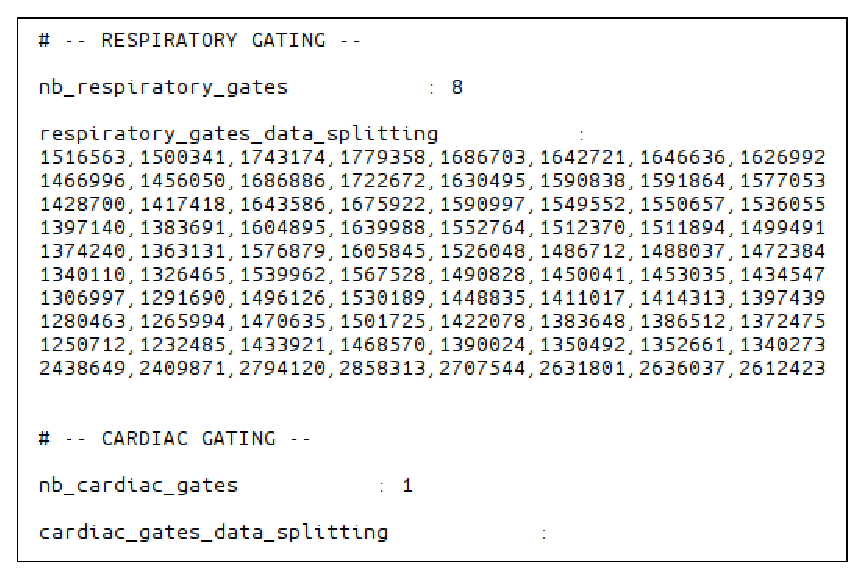
\includegraphics[width=0.8\columnwidth]{./figures/ex_gate_file.eps}
\caption{Set up of a gating file related to a dynamic dataset with respiratory gating}
\label{fig_ex_gate_file}
\end{figure}



\clearpage
\section{Dynamic model initialization}
A dynamic model module can be enabled in order to perform temporal based processing, such as kinetic modelling or temporal regularization, between the images of each frame (or gate).

The \textbf{-dynamic-model} command line option allows to specify a dynamic model and its potential configuration parameters (see details in section \ref{section_Meta-data command line options}). CASToR currently contains a \textit{LinearModel} class, and a \textit{Patlak} class dedicated to kinetic modelling for irreversible radiotracers. Both class are described in the following sections. More details about the available dynamic models and information regarding their initialization can be displayed using the command \textbf{-help-dmodel}. 




\subsection{iLinearModel:}
\label{ss_lmodel}


This class implements a general linear dynamic model applied between the images of a dynamic acquisition. The model is applied on a voxel-by-voxel basis between either the images of the frames or respiratory / cardiac gates. Several models could be used simultaneously on 5D/6D datasets (i.e dynamic gated acquisitions splitted in chronological time frames, or dual-gated acquisitions). At each iteration and subset, the parametric images of the model, and optionally the basis functions of the model, are estimated using the nested EM algorithm. Several variables control different parameters of the algorithm, such as the number of iterations of EM iterations for the model, the ratio of parametric images updates before basis function updates. This class must be initialized using a configuration file with the following command-line option: 

\bigskip
\verb| -dynamic-model LinearModel:/path/to/conf/file.txt|
\bigskip

The configuration file must contain one (or several) couple(s) of BEGIN/END keywords to define at which dynamic level of modelling the user-provided parameters must be applied:
\begin{itemize}
\item DYNAMIC FRAMING / ENDDF : model related to the chronological dynamic frames of the dynamic dataset
\item RESPIRATORY GATING / ENDRG : model related to the respiratory gates of the dynamic dataset
\item CARDIAC GATING / ENDCG : model related to the cardiac gates of the dynamic dataset
\end{itemize}


The following parameters could be defined inside these keywords to set a dynamic model at a specific dynamic level:
\begin{itemize}

\item \textbf{Number basis functions: x}	(mandatory) 

The number \textit{x} of basis functions (and parametric images) defined in the model

\item \textbf{Basis functions: list}	(mandatory)
 
Basis function initial values (list of coefficients for each frame or gate, separated by commas. Each functions must be entered on new lines)

\item \textbf{Parametric images init: path} (optional) 

Parametric images initialization using an interfile image located at the provided \textit{path}. Without initialization, all voxel will be set to 1 by default)

\end{itemize}


\bigskip
The following parameters are common to all level of dynamic models:


\begin{itemize}
\item \textbf{Number model iterations: x}	

Number of iterations of the model parameters and basis functions updates in one cycle of Nested EM (one cycle consists in x iterations in which either the parametric images or the basis functions are updated) (Default x ==  1)
   
\item \textbf{Basis function update ratio: x}	

Ratio of update between parametric images and basis functions updates cycle. Cycles consist in x iterations of the parametric images, following by x iterations of the basis functions. If x == 0, only the parametric images are updated (Default x ==  0).
          
\item \textbf{Basis function start ite : x}	

Starting iteration for the update of basis functions. If negative, no update of the basis functions is performed (only parametric images are updated) (Default x == -1).                                                                        
\end{itemize}

\begin{lstlisting}[label={sample},caption= Example of LinearModel initialization.]

   DYNAMIC FRAMING
   Number basis functions         : 2
   Basis_functions            :
   23682.79, 25228.74, 26636.99, 27923.61, 29101.16
   5.4, 4.91, 4.48, 4.1, 3.75
   ENDDF
   
   RESPIRATORY GATING
   Number basis functions         : 6
   Basis_functions            :  
   1, 0.8, 0.6, 0.4, 0.2, 0.01
   0.7, 0.9, 0.7, 0.5, 0.3, 0.1
   0.4, 0.6, 0.8, 0.6, 0.4, 0.2
   0.2, 0.4, 0.6, 0.8, 0.6, 0.4
   0.1, 0.3, 0.5, 0.alpin7, 0.9, 0.7
   0.01, 0.2, 0.4, 0.6, 0.8, 1
   ENDRG
   
   Number_model_iterations : 1
   Basis_function_start_ite : -1
   Basis_function_update_ratio : 0

\end{lstlisting}      
















\subsection{iLinearPatlakModel:} 
\label{ss_patlak}

This class implements the Patlak Reference Tissue Model (Patlak CS, Blasberg RG: Graphical evaluation of blood-to-brain transfer constants from multiple-time uptake data. J Cereb Blood Flow Metab 1985, 5(4):5 84-590. DOI http://dx.doi.org/10.1038/jcbfm.1985.87)
 
It is used to model radiotracers which follows as 2-tissue compartment model with irreversible trapping. The Patlak temporal basis functions are composed of the Patlak slope (integral of the reference TAC from the injection time divided by the instantaneous reference activity), and intercept (reference tissue TAC). 
   


It can be initialized using either a configuration file or a list of option with the following keywords and information:

\subsubsection{configuration file:} 
\label{sss_patlak_cfile} 
 
The file must be provided to the \textit{castor-recon} main executable using the following command-line options.

\bigskip
\verb| -dynamic-model Patlak:/path/to/conf/file.txt|
\bigskip

As this class inherits from the \textit{LinearModel} class. The parameters must be declared inside a couple of the following specific tags:
 
  - DYNAMIC FRAMING/ENDDF 


The following parameters must be defined inside these keywords to set a dynamic model at a specific dynamic level:

\begin{itemize}

\item \textbf{Basis functions: list}	(mandatory)
 
The coefficients of Patlak plot and intercept for each time frame (tf), on two successive lines, separated by ',' :
Basis functions: 
coeffPplottf1, coeffPplottf2, ..., coeffPplottfn
coeffPintctf1, coeffPintctf2, ..., coeffPintctfn


\item \textbf{Parametric images init: path} (optional) 

Parametric images initialization using an interfile image located at the provided \textit{path}. Without initialization, all voxel will be set to 1.0 and 1000. for the Patlak slope and intercept by default)


\item \textbf{Patlak method: x} (optional) optimization method for Patlak parameters estimation: 
x=0: Least-Square (default) 
x=1: Iterative non-negative Least-Square (C.L. Lawson and R.J. Hanson, Solving Least Squares Problems)
x=2: Nested EM (todo )
\end{itemize}


\subsubsection{Command line options:} 
\label{sss_patlak_list} 

The Patlak class initialization can be directly made from the command line options. Thelist of options must contain the coefficients of both Patlak functions separated by commas, with the following template :

\bigskip
\verb| -dynamic-model Patlak,coeffPplottf1,coeffPplottf2,...,coeffPplottfn,|

\verb|                coeffPintctf1,coeffPintctf2,...,coeffPintctfn|
\bigskip

The parametric images will be initialized with 1.0 and 1000. for Patlak slope and intercept by default. The parametric images estimations will be written on disk for each iteration. Default optimization method is least-square.
      
   
   
  
\subsection{Parameters common to all dynamic model:} 
\label{ss_common_parameters}

The following keywords are optional and common to each dynamic model (Dynamic frame, Respiratory gating or Cardiac gating). They control the main functions dedicated to the estimation of the model parameters, and the re-estimation of the image using the model:

\begin{itemize}
\item \textbf{Number of iterations before image update: x}  

Set a number \textit{x} of iteration to reach before using the model to generate the images at each frames/gates (Default x ==  0) 
   
\item \textbf{No image update: x } 

If \textit{x} set to 1, the reconstructed images for the next iteration/subset are not reestimated using the model (the code just performs standard independent reconstruction of each frames/gates) (Default x = 0).       
          
\item \textbf{No parameters update: x} 

If set to 1, the parameters / functions of the model are not estimated with the image (this could be used to test The EstimateImageWithModel() function with specific user-provided parametric images) (Default x = 0).
   
\item \textbf{Save parametric images : x } 

Enable (1)/Disable(0) saving parametric images on disk (Default x == 1)  
\end{itemize}




\clearpage
%---------------------------------------------------------------------------------------------------------------------------------------------------------------
\section{The dynamic module architecture}

The main classes managing dynamic models are \textit{oDynamicModelManager} and \textit{vDynamicModel}, located in the dynamic subfolder. The main program will instantiate and initialize the \textit{oDynamicModelManager} and the dynamic model class inheriting from \textit{vDynamicModel} if enabled. During the iterative reconstruction process, at the end of each iteration/subset loop, the \textit{ApplyDynamicModel()} function of the manager will call the \textit{EstimateModel()} and \textit{EstimateImage()} functions. The first will successively call the \textit{EstimateModelParameters()} and \textit{EstimateImageWithModel()} functions of the child class. As their names suggest, the first function is dedicated to the estimation of any parameters of the model, while the second function is used to regenerate an image from the model. The addition of a new dynamic model mostly require to implement these two functions. Note that these functions can be individually enabled/disabled depending on the values of some parameters implemented by \textit{vDynamicModel} specific to vDynamicModel as specified in section \ref{ss_common_parameters}. Please have a look to the next section \ref{section_add_own_dynamic_model} for more help about the dynamic model implementation itself.




\clearpage
%---------------------------------------------------------------------------------------------------------------------------------------------------------------
\section{Add your own dynamic model}
\label{section_add_own_dynamic_model}

\subsection{Basic concept}

The addition of a new image-based dynamic model require to build a specific class that inherits from the abstract class \textit{vDynamicModel}. Then, one just has to implement a set of pure virtual functions for the initialization and application of the model. Please refer to the \textit{CASToR\_HowTo\_\_add\_new\_modules.pdf} guide in order to fill up the mandatory parts of adding a new module; namely the auto-inclusion mechanism, the interface-related functions and the management functions. To ease the implementation, a template class is provided in the source code and already implements all the squeleton. Basically, one will have to change the name of the class and fill the related functions up in his own code. The actual files are \textit{include/dynamic/iDynamicModelTemplate.hh} and \textit{src/dynamic/iDynamicModelTemplate.cc} and are actually already part of the source code. Right below are some instructions to help fill the specific pure virtual projection functions of a dynamic model.
\bigskip


\subsection{Implementation of the dynamic model functions}

Several mandatory functions should be implemented (or return an error by default) in a new dynamic model class :

\begin{description}
\item \textbf{ShowHelp()}: Simply output some help and guidance to describe what the dynamic model does and how to use it.
\item \textbf{ReadAndCheckOptionsList()}: Implement here the reading of any options specific to this dynamic model passed through the argument \texttt{const string\& a\_listOptions}. The user can make use of the \textit{ReadStringOption()} function to parse the list of parameters. If the function is not mandatory (e.g initialization of the model using a file is required rather than with command-line parameters), just send an error message and return 1.
\item \textbf{ReadAndCheckConfigurationFile()}: Implement here the reading of any configuration file specific to this dynamic model, passed through the argument \texttt{const string\& a\_fileOptions}. The user can make use of the \textit{ReadDataASCIIFile()} function to read data from a file. If the function is not mandatory (e.g initialization of the model using command line options is required rather than with a file), just send an error message and return 1.
\item \textbf{CheckParameters()}: Use this function to check if the private parameters of your class have correctly been initialized. It might be a good idea to initialize all private parameters in the constructor with default erroneous value to properly check their initialization.
\item \textbf{InitializeSpecific()}: Use this function to Instanciate/Initialize any member variables/arrays after the parameters have been checked in the previous function.
  
\item \textbf{EstimateModelParameters()}: The estimation of the model parameters and parametric images must be implemented here, with the help of any private functions if required. The \textit{ap\_ImageS} parameter allows to access the image matrices in the oImageSpace class. The current estimation of the image \textit{m4p\_image} can be accessed from there. It contains 4 dimensions in order to access to any dynamic level : 

$ap\_ImageS->m4p\_image[fr][rg][cg][v]$ \\
fr = time frames \\
rg = respiratory gates \\
cg = cardiac gates \\
 v = actual voxel of the 3D volume

\item \textbf{EstimateImageWithModel()}: This function can be used to generate the serie of dynamic images from the model (i.e, the image matrix $ap\_ImageS->m4p\_image$), after estimation of the model parameters in EstimateModelParameters(). It is called right after EstimateModelParameters()

All information and the tools needed to implement these functions are fully described in the template source file \textit{src/dynamic/iDynamicModelTemplate.cc}, so please refer to it.

\end{description}



\section{castor-ImageBasedDynamicModel toolkit}
\label{section_dmodel_toolkit}

// TODO



\clearpage
\section{Meta-data command line options}
\label{section_Meta-data command line options}
List of the different set of options related to image-based dynamic models :
\begin{itemize}
\item \textbf{-g} \textit{file}: Give a text file defining the dynamic data splitting (due to respiratory/cardiac gating or involuntary patient motion correction).
      The file should contain the some of the following keywords :
\begin{description}
\item \texttt{nb\_respiratory\_gates}: number of respiratory gates in the data
\item \texttt{respiratory\_gates\_data\_splitting}: enter the number of events within each gate, separated by commas. If the data contains several frame (dynamic
      acquisition), the data splitting of each frame should be entered on a new line
\item \texttt{nb\_cardiac\_gates}: number of cardiac gates in the data
\item \texttt{cardiac\_gates\_data\_splitting}: enter the number of events within each gate, separated by commas. If the data contains several frame (dynamic
      acquisition), the data splitting of each frame should be entered on a new line.
\item \texttt{nb\_involuntary\_motion\_triggers}: number of involuntary patient motion triggers in the data
\item \texttt{listt\_involuntary\_motion\_triggers}: enter the timestamp of each transformation, separated by commas. No specific nomenclature is required for dynamic acquisitions (data containing several frames). However, if the data contains several bed positions, the data splitting of each bed should be entered on a new line.
\end{description}
\item \textbf{-rm} \textit{param}: Give the deformation to be used for respiratory motion correction, along with a configuration file (deformationModel:file), or the list of parameters associated to the deformation model (deformationModel,param1,param2,...).
\item \textbf{-cm} \textit{param}: Give the deformation to be used for cardiac motion correction, along with a configuration file (deformationModel:file), or the list of parameters associated to the deformation model (deformationModel,param1,param2,...).
\item \textbf{-rcm} \textit{param}: Give the deformation to be used for dual gating motion correction (both respiratory and cardiac), along with a configuration file (deformationModel:file), or the list of parameters associated to the deformation model (deformationModel,param1,param2,...).
\item \textbf{-im} \textit{param}: Give the deformation to be used for patient motion correction, along with a configuration file (deformationModel:file), or the list of parameters associated to the deformation model (deformationModel,param1,param2,...).
\end{itemize}


%---------------------------------------------------------------------------------------------------------------------------------------------------------------
%---------------------------------------------------------------------------------------------------------------------------------------------------------------
%---------------------------------------------------------------------------------------------------------------------------------------------------------------
%          R E F E R E N C E S
%---------------------------------------------------------------------------------------------------------------------------------------------------------------
%---------------------------------------------------------------------------------------------------------------------------------------------------------------
%---------------------------------------------------------------------------------------------------------------------------------------------------------------
\bibliographystyle{IEEEtran} 
%\bibliographystyle{apalike} 
\bibliography{CASToR_general_documentation}

% that's all folks
\end{document}
